\documentclass[aspectratio=169, t, 10pt,
    ignorenonframetext,
    ]{beamer}
\usetheme{Boadilla}
\beamertemplatenavigationsymbolsempty

\usepackage{standalone}
\usepackage[utf8]{inputenc}
\usepackage[english]{babel}
\usepackage{pgfplots}
\usepackage{mathtools}
\mathtoolsset{showonlyrefs}
\usepackage{qrcode}
\usepackage{multimedia}

\newcommand\Mean[1]{\mathbb{E}\!\left[#1\right]}
\newcommand\Var[1]{\mathbb{V}\!\left[#1\right]}
\newcommand\Cov[2]{\mathrm{Cov}\!\left[#1,#2\right]}
\newcommand\Gauss[2]{\mathcal{N}\!\left({#1},\,{#2}\right)}
\newcommand\GP[2]{\mathcal{GP}\!\left({#1},\,{#2}\right)}
\newcommand{\Identity}{\mathbb{I}}

\title[Correlation based travel time inversion]{Bayesian Travel Time Inversion adopting Gaussian Process Regression}
\subtitle{-- with a focus on uncertainty analysis --}
\author[\tt mauerber@uni-potsdam.de]{Stefan Mauerberger \and Matthias Holschneider}
\institute[Math@UP]{University Potsdam, Institute of Mathematics}
\titlegraphic{%\vspace{-1cm}
              \hspace{2cm}
              \parbox[c]{0.17\linewidth}{
\includegraphics[width=\linewidth]{./logos/GeoSim_Logo}}
              \hfill
              \parbox[c]{0.10\linewidth}{
\includegraphics[width=\linewidth]{./logos/UniPotsdam_Logo}}
              \hspace{2cm}
              }
\date[AGU~2017]{AGU Fall Meeting -- 13\textsuperscript{th} December 2017}

\input{def_example}
\begin{document}

\frame[noframenumbering, plain]
    {\maketitle}

~

\begin{frame}
    \frametitle{Travel Time Tomography}
    \framesubtitle{~}%
%
\begin{columns}%
\column{.55\textwidth}%
%
    \begin{itemize}
        \item Bayesian inversion
        \item Correlation based
        \item Non parametric
    \end{itemize}

    \begin{exampleblock}{Synthetic test}
        \begin{itemize}
            \item Large scale anomalies as a reference model
            \item Neglecting dispersion and refraction
            \item Station geometry borrowed from ScanArray
        \end{itemize}
    \end{exampleblock}

    \begin{alertblock}{Infer reference model from travel time obs.}
        Bayesian posterior distribution \\
        \hfill {\Large $\leadsto$} Location dependent model uncertainties ~
    \end{alertblock}

\column[T]{.44\textwidth}
    \vspace{-10mm}
    \input{fig_reference_model.pgf}
\end{columns}

\end{frame}

I am providing new insight into travel time tomography from a correlation based point of view.
\\
The objective is to retrieve the velocity model posterior to travel time observations.
\\[2mm]

To carry on with a synthetic test a subset of $\SFWnst$ stations of the ScanArray is considered.
\\
The reference model is composed of two large scale anomalies.
\\
Travel times are generated from that model neglecting refraction and dispersion.
\\
The aim of the example is to recover the reference model;
In particular its uncertainties.


\begin{frame}
    \frametitle{Travel Time Observations}
    \framesubtitle{a non-linear functional w.r.t.~the velocity model}

\begin{columns}
\column{.55\textwidth}%
    \begin{equation}
        \mathrm T_C[v] = \int_C \frac 1{v(r)} \mathrm d r
    \end{equation}

    \begin{description}[leftmargin=! ,labelwidth=1cm]
        \item [Observational functional] $\mathrm T_C[\,\cdot\,]$
        \item [Ray path]                 $C_{s,r}[\,\cdot\,]$
        \item [Source location]          $s$
        \item [Receiver position]        $r$
        \item [Velocity model]           $v$
    \end{description}

    \begin{alertblock}{It is the velocity model what we are after}
    \begin{itemize}
        \item Travel times are putting an Integral-constraint on $v$
        \item Non-linearity is a major concern
    \end{itemize}
    \end{alertblock}


\column[T]{.44\textwidth}
    \vspace{-10mm}
    \only{\input{fig_path_coverage.pgf}}
    \small
    \begin{align}
        N_\text{stn} &= \SFWnst &
        & \leadsto &
        N_\text{obs} &= \SFWnobs
    \end{align}

\end{columns}

\end{frame}

Travel times are expressed in terms of an integral over the slowness along the ray path.
\\
The observational functional is putting an integral constraint on the velocity model.
\\
However, the non-linear relation of travel times and velocity model is a challenge.
\\[2mm]

In the example, travel times are calculated for all station pairs, totaling to a $\SFWnobs$ records.
\\
Measurement noise is simulated by drawing from a normal distribution.
\\[2mm]

Before going ahead with non-linearity lets have a look at the a\,priori assumptions.


\begin{frame}
    \frametitle{A\,Priori Velocity Model}
    \framesubtitle{expressing our ignorance}

\begin{columns}
\column{.55\textwidth}%
    \begin{block}{Assume the model a Gaussian Random Field}
    \begin{equation}
        v \to V \sim \GP{\mu_V}{K_V}
    \end{equation}
    \begin{description}[leftmargin=! ,labelwidth=6cm]
        \item [Prior mean function] $\mu_V(x) = \SFWmuCpri \, \frac ms$
        \item [Covariance function] $K_V(x,y)$
    \end{description}
    \end{block}
    \medskip

    Assumed covariance
    \begin{equation}
        K_V(x,y) = \tau^2 \exp\left\{ -\frac12 \frac{d(x,y)^2}{\ell^2}\right\}
    \end{equation}
    \begin{description}[leftmargin=! ,labelwidth=6cm]
        \item [Great circle distance] $d(x,y)$
        \item [Standard deviation]   $\tau = \SFWtau \, \frac ms$
        \item [Characteristic length]  $\ell = \SFWell \, m$
    \end{description}

\column[T]{.44\textwidth}
    \centering
    \vspace{-10mm}
    \input{fig_kernel_pri.pgf}

\end{columns}

\end{frame}

To express our ignorance, the a\,priori velocity model is assumed a Gaussian random field.
\\
It is fully determined by its mean function and covariance function.
\\[2mm]

For the example, a constant prior mean of $\SFWmuCpri \, \frac ms$ is used.
\\
The chosen covariance is inspired by the squared exponential kernel.
\\
The characteristic length is $\SFWell \, m$ and the deviation from the mean is $\SFWtau \, \frac ms$.
\\[2mm]

The kernel is depicted on the right.
\\
The further two points are apart the less correlated they are.
\\
In turn, close by points are likely to share similar velocities.


\begin{frame}
    \frametitle{Linearization}
    \framesubtitle{Gaussianity is preserved under linear maps}

\begin{columns}
\column{.55\textwidth}%
    \begin{equation}
        \mathrm T_C[V] \approx \int_C \frac 1{\mu_V(r)} - \frac{V(r)}{\mu_V(r)^2} \, \mathrm d r
    \end{equation}
    \begin{description}[leftmargin=!, labelwidth=1cm]
        \item [Taylor expansion] 1\textsuperscript{st} order
        \item [point of expansion] $\mu_V$ (prior mean)
    \end{description}
    \medskip

    \begin{block}{Approximated correlation}
    \begin{equation}
        \Cov{V}{\mathrm T_C[V]\,} \approx -\int_C \frac {K_V(\cdot,r)}{\mu_V(r)^2} \, \mathrm d r
    \end{equation}
    \end{block}

    \begin{block}{Approximated co-variance}
    \setlength\abovedisplayskip{0pt}
    \begin{equation}
        \Cov{\mathrm T_C[V]}{\mathrm T_{C'}[V]\,} \approx  \int_C \int_{C'} \frac{K_V(r,r')}{\mu_V(r)^2\mu_V(r')^2} \, \mathrm d r \, \mathrm d r'
    \end{equation}
    \end{block}

\column[T]{.44\textwidth}
    \centering
    \vspace{-10mm}
    \input{fig_correlation_pri.pgf}
    \\ \scriptsize
    ~~ Correlation of $V(x)$ with $T_C[V]$ kept fix

\end{columns}

\end{frame}

In case of non-linearities, it is not feasible to calculate the full Bayesian posterior.
\\
To preserve Gaussianity a Taylor expansion around the prior mean function is preformed.
\\
The linearization turns correlations and co-variances into explicit formulas.
\\[2mm]

The figure on the right shows what is learned about the medium from a single measurement.
\\
In other words: If we consider the travel time for a certain path, the intensity of the color describes its influence on the model.


\begin{frame}
    \frametitle{Bayesian Posterior Distribution}
    \framesubtitle{Gaussian Process Regression}

\begin{columns}
\column[t]{.48\textwidth}

    \begin{block}{Stochastic data model}
        \begin{equation}
            D = \mathrm T_C[V] + E \sim \Gauss{\mu_D}{\Sigma_{DD}}
        \end{equation}
        \begin{description}[labelwidth=25mm]
            \item [Error model]        $E\sim \Gauss{0}{\sigma_\varepsilon^2}$
            \item [Uncertainty]        $\sigma_\varepsilon = \SFWepsilon\,s$
            \item [Prior travel times] $\mu_D = \Mean{\mathrm T_C[\mu_V]\,}$
            \item [Covariance matrix]  $\Sigma_{DD} = \Cov{\mathrm T_C}{\mathrm T_{C'}} + \Identity \sigma_\varepsilon^2$
        \end{description}
    \end{block}

    \begin{itemize}
        \item The kernel spans a function space (RKHS)
        \item Sort out functions incompatible with data
    \end{itemize}

\column[t]{.48\textwidth}

    \begin{exampleblock}{Conditional mean and covariance}
        \setlength\abovedisplayskip{0pt}
        \begin{alignat}{3}
            \Mean{V|d} &= \mu_V &&+ \Cov VD \Sigma_{DD}^{-1} \big( d - \mu_{D} \big)
            \\
            \Var{V|d}  &= K_V   &&- \Cov VD \Sigma_{DD}^{-1} \Cov DV
        \end{alignat}
        \hfill {\Large $\leadsto$} Posterior distribution \phantom{p}
    \end{exampleblock}

    \begin{alertblock}{Accommodate non-linearity}
        \begin{itemize}
            \item Single evidence at a time
            \item Correlations and Variances from predecessor
        \end{itemize}
        \hfill {\Large $\leadsto$} Successive approach ~
    \end{alertblock}

\end{columns}

\end{frame}

A stochastic data model accounting for normal noise is chosen.
\\
Travel times are assumed being accurate at about $\SFWepsilon\,s$.
\\[2mm]

The posterior distribution is given by conditional mean and covariance.
\\
The basic grasp is to narrow down the function space to only those functions that are in accordance with the data.
\\[2mm]

To accommodate non-linearity I pursue with a successive strategy similar to a Kalman filter.
\\
The overall idea is to only incorporate a single evidence at a time.
\\
The linearization is performed at each step, again and again.
\\
Hereby the posterior mean improves gradually.
\\
The closer the point of expansion to reality the better the Taylor expansion performs.
\\[2mm]

\begin{frame}
    \frametitle{Successive Approach}
    \begin{center}
    \movie[height=0.85\textheight, width=1.51\textheight, autostart]{\includegraphics[height=0.85\textheight, width=1.51\textheight]{animation_pst}}{animation.avi}
    \end{center}
\end{frame}

To illustrate the idea, I prepared a little video.
\\
The left hand panel shows how the conditional mean develops.
\\
Contour lines are for comparison with the reference model.
\\
On the right, the evolution of the conditional standard deviation is depicted.
\\[2mm]

The path by path construction can nicely be seen.
\\
Both anomalies are captured.
\\
The characteristic length is refected by the extent of the patches.
\\
Areas of dense ray coverage are showing highes confidence gain.


\begin{frame}
    \frametitle{Conclusions \phantom{I}I/II}
    \framesubtitle{Assessment of Uncertainties}

\begin{columns}
\column{.55\textwidth}%

    \begin{itemize}
        \item Anomalies are captured
        \item Variance reduction $\Delta\sigma = \SFWsdred$
        \item Measurement accuracy is dominant factor
        \item Analogy with sensitivity kernels
        \item Posterior as superposition
    \end{itemize}

\column[T]{.44\textwidth}
    \vspace{-10mm}
    \only<1>{\input{fig_correlation_pst.pgf}}
    %\only<2>{\input{fig_correlation_pri.pgf}}

\end{columns}

\end{frame}


\begin{frame}
    \frametitle{Conclusions II/II}
    \framesubtitle{Data Misfit }

\begin{columns}
\column{.55\textwidth}%
    \begin{itemize}
        \item Data misfit
            \begin{equation}
                \phi = (d-\mu_D)^T \Sigma_{DD}^{-1} (d-\mu_D)
            \end{equation}
        \item Calculus in the function space view
        \item Effect of succession order
        \item Memory intense discretization
    \end{itemize}

    \begin{exampleblock}{Bayesian Posterior Distribution}
        Accommodates non-linearity
    \end{exampleblock}

\column[T]{.44\textwidth}
    \vspace{-10mm}
    \documentclass[beamer=true]{standalone}
\usepackage{pgfplots}
\input{def_example}
%
\begin{document}
\begin{tikzpicture}
    \pgfplotstableread{./dat/misfit.dat}\misfit
    \pgfplotsset{axis lines=left, tick label style={font=\tiny}, log ticks with fixed point}
    \begin{semilogyaxis}[width=\textwidth, height=\textheight,
             ylabel={Data misfit}, xlabel={\# evidence}, ylabel near ticks,
             legend cell align=left,  xlabel near ticks,
             legend style={only marks, draw=none, font=\footnotesize,
             at={(0,0)}, anchor=south west },
             label style={font=\scriptsize}, name=big ]
        \addplot [dashed, mark=*, blue , mark options={scale=0.5, solid}] table [x=evd, y=all] \misfit;
        \addlegendentry{all at once}
        \addplot [dashed, mark=*, red  , mark options={scale=0.5, solid}] table [x=evd, y=asc] \misfit;
        \addlegendentry{ascending $\sphericalangle$}
        \addplot [dashed, mark=*, green, mark options={scale=0.5, solid}] table [x=evd, y=dsc] \misfit;
        \addlegendentry{descending $\sphericalangle$}
        \addplot [dashed, mark=*, black, mark options={scale=0.5, solid}] table [x=evd, y=rnd1] \misfit;
        \addlegendentry{shuffle}
        \addplot [dashed, mark=*, black, mark options={scale=0.5, solid}] table [x=evd, y=rnd2] \misfit;
    \end{semilogyaxis}
    \begin{axis}[at=(big.north east), anchor=north east, width=0.5\textwidth, height=0.5\textwidth,
                 xmin={\SFWnobs-14}, xmax={\SFWnobs+3}]
        \addplot [dashed, mark=*, red  , mark options={scale=0.5, solid}] table [x=evd, y=asc] \misfit;
        \addplot [dashed, mark=*, green, mark options={scale=0.5, solid}] table [x=evd, y=dsc] \misfit;
        \addplot [dashed, mark=*, black, mark options={scale=0.5, solid}] table [x=evd, y=rnd1] \misfit;
        \addplot [dashed, mark=*, black, mark options={scale=0.5, solid}] table [x=evd, y=rnd2] \misfit;
    \end{axis}
\end{tikzpicture}
\end{document}


\end{columns}

\end{frame}

\begin{frame}
    \frametitle{Outlook \& Next Steps }
    \framesubtitle{Potential future application}

\begin{columns}
\column{.55\textwidth}%

    \begin{itemize}
        \item Poisson type kernel
        \item Estimation of hyper parameters
        \item Adaptive grid to facilitate refraction
    \end{itemize}

    \begin{block}{Surface Wave Tomography}
        \begin{itemize}
            \item Model phase velocities $v(\omega)$
            \item Use ambient noise records
            \item Frequency dependent kernel
                \begin{equation}
                    K(x,\omega; x', \omega') = \, ???
                \end{equation}
                accounting for dispersion
        \end{itemize}
    \end{block}

\column[T]{.44\textwidth}
    \centering
    \only<1>{\vspace{-12mm}
        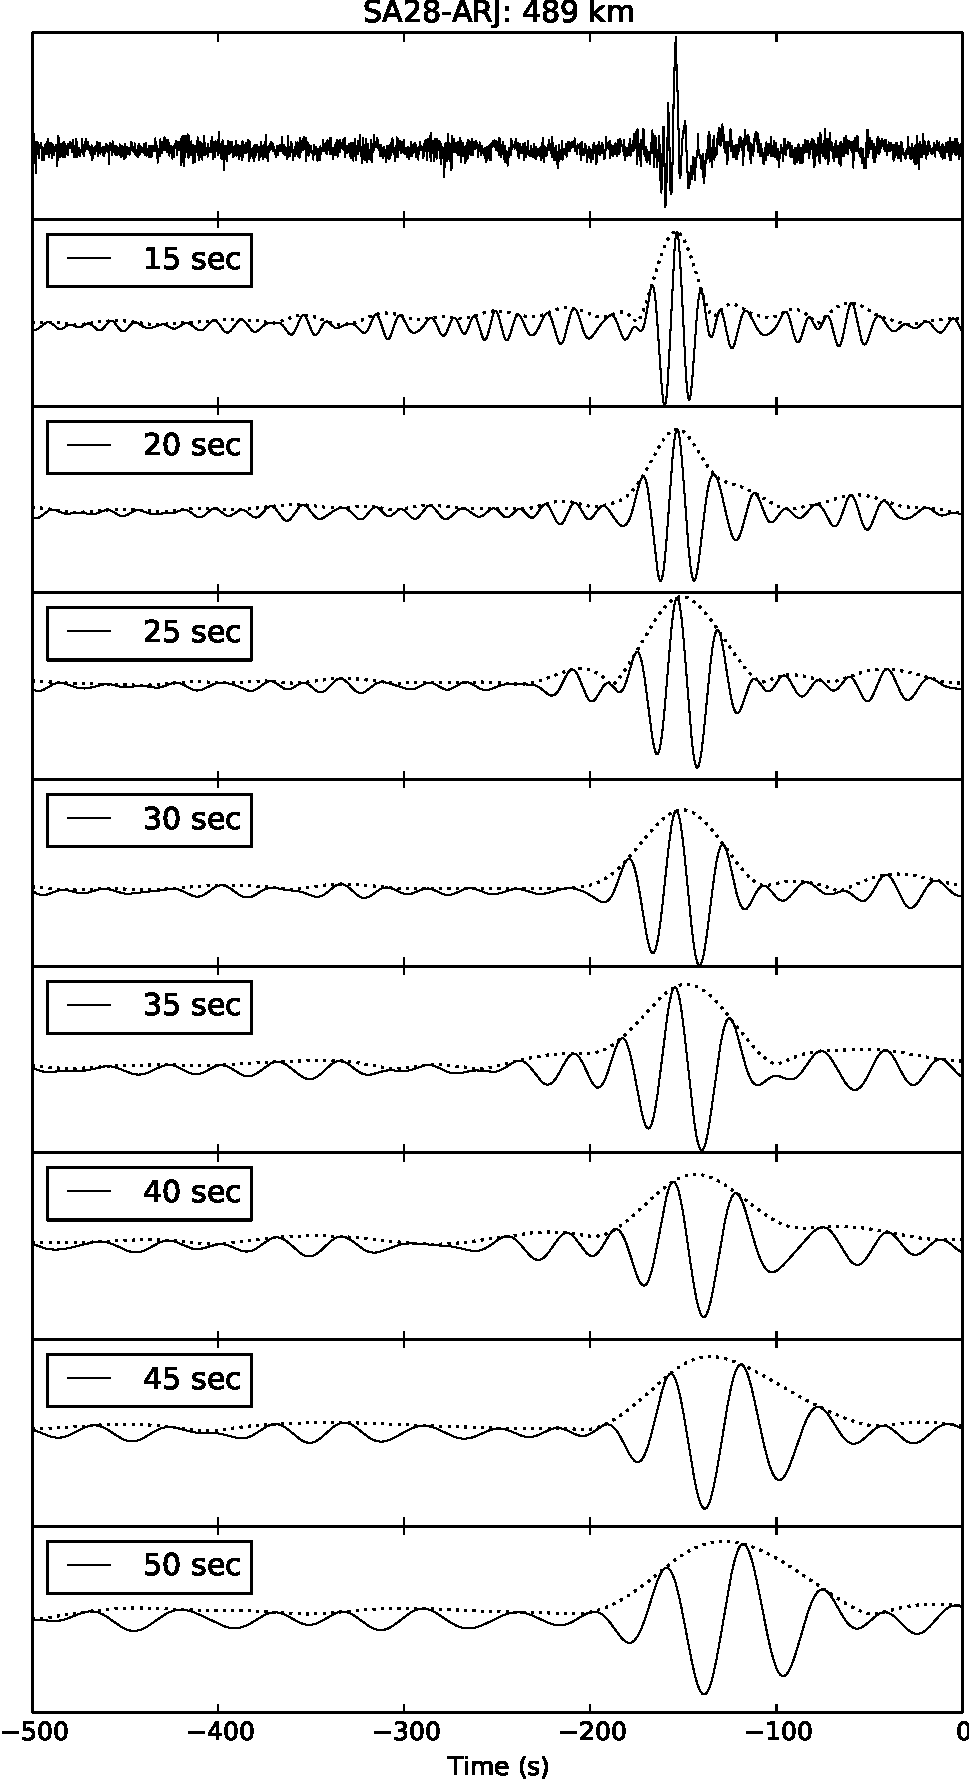
\includegraphics[height=0.9\textheight]{MultiFiltered_SA28-ARJ}
        \\
        \tiny Multi-filtered correlogram by courtesy of A.~Mauerberger
    }
    \only<2>{
        \vspace{2mm}
        Follow the project on GitHub
        \\[6mm]
        \fbox{\qrcode[height=3cm]{https://github.com/mauimuc/gptt}}
        \\[6mm]
        \small
        \href{https://github.com/mauimuc/gptt}{github.com/mauimuc/gptt}
    }
\end{columns}

\end{frame}

For spherical geometries the usage of a Poisson type kernel is natural.
\\
A maximum likelihood estimate appears adequate to guess prior mean and error level.
\\
However, NOT for the characteristic length.
\\[2mm]

Modeling phase velocities is a potential future application.
\\
Surface waves are showing strong dispersion, clearly visible in the correlogram on the right.
\\
To model phase velocities a frequency dependent kernel is required.
\\
A simple departure is a locally stationary kernel.
\\
Both characteristic length and variance are assumed to depend on the centroid and/or lag frequency.
\\[2mm]

Thanks for your attention; Looking forward to your questions.

\end{document}
